\documentclass[11pt,oneside,titlepage]{jsbook}

%%%--- Read Package ---%%%
\usepackage{times,array,fancyhdr,lastpage,amsmath,amssymb,txfonts,ccaption}
\usepackage{bm}
\usepackage[dvipdfm]{graphicx}
\usepackage[dvipdfmx]{color}
\usepackage[newitem,newenum]{paralist}%箇条書き書式変更スタイル
%\usepackage{slashbox}
\usepackage{bm}
\usepackage{here}
%\usepackage{subfigure}
\usepackage{comment}
\usepackage{type1cm}
\usepackage{amssymb}
\usepackage{cite}
\newcommand{\argmax}{\mathop{\rm max}\limits}

%%%--- Setup Layout ---%%%
\topmargin 0pt    %オフセットからヘッダまでのマージン
\headsep 35pt       %ヘッダと本文領域の間の高さ
\topskip 5pt        %本文領域内の本文開始位置までの高さ
\oddsidemargin 15pt %奇数ページのマージン
\footskip 30.00pt   %文章領域の終わりからフッタの終わりまでの高さ
\paperwidth 597pt   %用紙の幅
\paperheight 845pt  %用紙の高さ
\voffset 0pt        %垂直方向のオフセット
\hoffset 0pt        %水平方向のオフセット
\headheight 30pt    %ヘッダの高さ    
\evensidemargin 17pt%偶数ページのマージン
\marginparsep 10pt  %本文領域と傍注の間の幅
\marginparwidth 17pt%傍注の幅
\marginparpush 7pt  %傍注間の高さ
\textwidth 43zw     %文章領域の幅
\setlength{\textheight}{32.5\baselineskip}%行送り設定
\addtolength{\textheight}{\topskip}
\pagestyle{fancy}
\setcounter{tocdepth}{3}	%subsubsectionまでを目次に表示
\setcounter{secnumdepth}{4}

\begin{document}
\captiondelim{ }%キャプションの書式を変更
%↓fancy.styの設定
%\fancyhead{}
\rfoot{{\small 九州大学 大学院 システム情報科学府 情報知能工学専攻}}%右フッタ
%\fancyhead[LE]{\chaptermark}%偶数ページ左ヘッダ
%\fancyhead[LO]{\sectionmark}%奇数ページ左ヘッダ
\rhead{\textbf{\thepage}}   %右ヘッダ
\cfoot{}           %中央フッタ
\renewcommand{\headrulewidth}{0.4pt}
\renewcommand{\footrulewidth}{0.4pt}
\setlength{\baselineskip}{18.95pt}

%%%--- 章の最初のページのページ番号・ヘッダ・フッタを他のページと同じ形式で表示 ---%%% 
\makeatletter
\renewcommand{\chapter}{
  \if@openright\cleardoublepage\else\clearpage\fi
  \global\@topnum\z@
  \secdef\@chapter\@schapter}
\makeatother

%%%--- Title Page ---%%%
\vspace*{3cm}%\vspace*{長さ}:縦方向空白(ページ先頭有効)
\begin{center}%センタリングはじめ
{\Large \textbf{}}\\%\\:字下げ無し改行
\vspace{3mm}
{\Large \textbf{ベクトル符号化無線通信における\\送受信フィルタ係数の反復最適化}} \\
\vspace{5cm}%\vspace{長さ}:縦方向空白(ページ先頭無効)
\indent \\
{\Large 仁部龍介} \\
\vspace{5mm}
{\Large 平成 31年 2月} \\
\vspace{5mm}
{\Large 修士課程 \\ 情報知能工学専攻 \\ 社会情報システム工学コース} \\
\end{center}%センタリングおわり 
\thispagestyle{empty}%\thispagestyle{ページスタイル名}:一時的にページスタイル変更
           %empty:ページ番号無し,plain:フッタ中央にページ番号を付ける

%\clearpage %\clearpage(改ページ)		

%\chapter*{概要} %章番号をつけない
\thispagestyle{empty}

\thispagestyle{empty}
近年のスマートフォンやタブレット等の通信端末の急激な増加により通信トラフィックの増加が問題と
なっている.
これに対してシステム容量の拡大が喫緊の課題とされているが,
通信の高速化を阻害する要因としてチャネル歪みがある.このチャネル歪みに対して強い耐性を
もつ直交周波数分割多重(OFDM)方式が無線LANやディジタルテレビ放送等に幅広く用いられている.
OFDM方式は,周波数領域において直交する狭帯域なサブキャリアを用いた多重伝送を特徴とする.
この狭帯域性がチャネル歪みに対する強いチャネル耐性を実現する.

このOFDM方式に対して,ある状況においてより優れた伝送特性を示す変調方式としてベクトル符号化(VC)
がある.VCは伝搬路行列とその整合フィルタからなる合成チャネル行列の固有ベクトルを拡散符号とする
符号分割多重(CDM)方式である.合成チャネル行列はエルミート行列となるため,その固有ベクトルは
互いに直交する.また,受信側に整合フィルタを置くことで遅延派の取りこぼしのない
パスダイバーシチを実現できる.拡散符号の獲得に関して,これまでチャネル推定を用いた方法が検討されてきたが,
チャネル推定や推定した情報から固有値分解する必要があるため,膨大な演算量が必要となる.

そこで,この演算量を簡単な非線形処理と無線機間反復で代替するPing-Pong-Loop(PPL)を提案している.
PPLはべき乗法を基本原理とし,任意ベクトルを無線機間で往復
させることで徐々に固有ベクトルに収束させる点を特徴とする.しかし,PPLによる固有ベクトルの獲得には
ある程度の無線機間反復数が必要になるという課題がある.また,VC自体にも小さい固有値に対応する
チャネルを使用する場合,誤り率が高くなるという課題がある.本論文では,この2つの課題に対して
チャネルの足切りアルゴリズムと送信電力制御というアプローチを試みた.また,送信電力制御を
足切りアルゴリズムに適用することによって,使用可能チャネルを最大化しつつ無線機間反復数を
削減できることを,シミュレーションを用いて検証した.

\frontmatter %ページ番号はローマ数字、章番号をつけない
\clearpage %\clearpage(改ページ)

\chapter*{概要} %章番号をつけない
\thispagestyle{empty}

\thispagestyle{empty}
近年のスマートフォンやタブレット等の通信端末の急激な増加により通信トラフィックの増加が問題と
なっている.
これに対してシステム容量の拡大が喫緊の課題とされているが,
通信の高速化を阻害する要因としてチャネル歪みがある.このチャネル歪みに対して強い耐性を
もつ直交周波数分割多重(OFDM)方式が無線LANやディジタルテレビ放送等に幅広く用いられている.
OFDM方式は,周波数領域において直交する狭帯域なサブキャリアを用いた多重伝送を特徴とする.
この狭帯域性がチャネル歪みに対する強いチャネル耐性を実現する.

このOFDM方式に対して,ある状況においてより優れた伝送特性を示す変調方式としてベクトル符号化(VC)
がある.VCは伝搬路行列とその整合フィルタからなる合成チャネル行列の固有ベクトルを拡散符号とする
符号分割多重(CDM)方式である.合成チャネル行列はエルミート行列となるため,その固有ベクトルは
互いに直交する.また,受信側に整合フィルタを置くことで遅延派の取りこぼしのない
パスダイバーシチを実現できる.拡散符号の獲得に関して,これまでチャネル推定を用いた方法が検討されてきたが,
チャネル推定や推定した情報から固有値分解する必要があるため,膨大な演算量が必要となる.

そこで,この演算量を簡単な非線形処理と無線機間反復で代替するPing-Pong-Loop(PPL)を提案している.
PPLはべき乗法を基本原理とし,任意ベクトルを無線機間で往復
させることで徐々に固有ベクトルに収束させる点を特徴とする.しかし,PPLによる固有ベクトルの獲得には
ある程度の無線機間反復数が必要になるという課題がある.また,VC自体にも小さい固有値に対応する
チャネルを使用する場合,誤り率が高くなるという課題がある.本論文では,この2つの課題に対して
チャネルの足切りアルゴリズムと送信電力制御というアプローチを試みた.また,送信電力制御を
足切りアルゴリズムに適用することによって,使用可能チャネルを最大化しつつ無線機間反復数を
削減できることを,シミュレーションを用いて検証した.

%\pagenumbering{roman}
\tableofcontents %目次出力
\rhead{}

\mainmatter %ページ番号は算用数字、章番号をつける

\newpage
\rhead{\thepage}
\chapter{序論}
 
近年,スマートフォンやタブレット等の通信端末の急激な増加に伴い,大容量通信への期待が高まっている.
これを実現する有望な方策は小型の無線基地局を面的に多数設置し,面的周波数利用効率を高めること
である.しかしながら,無線基地局を多数設置するには基幹回線に接続するための有線バックホール回線を
要するため,その敷設コストの増大が問題となる.
そのため,バックホールとして無線中継網を用いる手法が検討されている~\cite{yamo} \cite{pabst}.
 ところで,一般的に,無線回線において高速伝送を行う場合,受信信号には遅延波による符号間干渉
 (信号歪み)が発生するため,適応等化等の信号歪みのへ対策技術が必須となる~\cite{akaiwa}.
 無線中継網の中継回線は端末の移動を伴うアクセス回線と比べて比較的静的であるため,
 その中継回線品質を高めるには送信機と受信機の双方で適応等化を行うことが有効である.

 線形フィルタを用いて送受信等化を実現する技術として,ベクトル符号化(\emph{VC:Vector Coding})~\cite{kasturia}が
知られている.ベクトル符号化は伝搬路相関行列の固有ベクトルを重み係数とする線形フィルタを
送受信で用いる方式であり,非線形の信号処理を行うことなく,信号電力対雑音電力比の最大化と
無歪み伝送(符号間干渉無し)を可能とする.また,無線LANや携帯電話システム等で広く採用されている
直交周波数分割多重(\emph{OFDM: Orthogonal Frequency Division Multiplexing})方式と異なり,
誤り訂正符号化を行うことなくパスダイバーシチ効果を得ることができるため~\cite{furukawa},
無線中継網等の固定回線通信においてはベクトル符号化がOFDMよりも優れた伝送特性を示すことが
期待できる.~\cite{furukawa,li,takeda,takanashi}しかしながら,ベクトル符号化を行うには送受信機双方でチャネル情報が必要となるため[**],
チャネル推定とその固有値分解に非常に多くの演算が必要になる~\cite{takano} \cite{takeda2}.
これは,演算能力が限られた小型中継機を用いる場合,大きな制約となる.従来,べき乗法~\cite{strang}の原理に
基づき,固有値分解の演算を簡易な非線形処理と無線機間反復処理に置き換えるPing-Pong-Loop(PPL)が
提案されている.PPLは,任意ベクトルを2つの無線機間で反復処理することで,
徐々に合成チャネル行列の固有ベクトルに収束させる点を特徴とする.
しかしながら,PPLを用いることで送受信機の個々の演算量は軽減されるものの,
反復演算の収束値を得るために,特に固有値が小さい固有ベクトルを求めるために多大な無線機間反復を
こなす必要があり,解決すべき課題となる.
また,小さい固有値に対応する固有チャネルでは,チャネル利得が固有値の大きさに応じて小さくなることから,
比較的誤りやすくなるという課題がある.

本論文では,PPLにおける上記の課題を解決するために,以下の検討を行う.
第1に,獲得すべき固有ベクトル数を考慮したPPLにおける反復停止規範を提案する.
通信品質が基準以下である固有ベクトルに関してPPLの反復処理を停止することで,
獲得すべき固有ベクトルの足きりを行うものである.PPLアルゴリズムはべき乗法に基づくため,
固有値が小さい場合ほど収束が遅い. 提案方式では,固有値とBERの理論的な関係からPPLの反復毎に
BERを求め,それが所要値以下となる場合に演算を停止する.
それにより,不要な固有ベクトルを獲得する必要がないため,無線機間反復数を削減することができる.
第2に,PPLのための送信電力分配法を提案する.BER最少化規範に基づき送信電力を
各固有チャネルに最適分配することで利得の小さい固有チャネルの誤り率の改善を行う.
最後に,送信電力分配と足切りアルゴリズムを併用することで,反復回数を抑えながら,
一定の通信品質を満足するチャネル数の最大化を行う.

 本論文は以下のように構成される.第2章では提案手法の原理を支える数学的基礎概念と
ディジタル通信に関する基礎概念を説明する.第3章では提案アルゴリズムの根幹となるPPL過程について
説明を行い, 第4章にて本論文における検討方式の説明とシミュレーションによる検証を行う.
最後に第5章において,本論文のまとめと今後の展望について述べる.
 %序論
\chapter{基本的概念の解説}
本章では,本論文を理解する上で必要となる基本概念についての説明を行う.VCを理解するため材料として
エルミート行列の性質やべき乗法について説明する. \cite{strang} また,無線通信の理解に関してディジタル変復調,
同期検波等について説明を行う.

\section{数学的基礎知識}
VCを理解するための事前準備として数学的基礎知識の説明を行う.本章では行列の要素が複素数である
複素行列を扱っている.

\subsection{随伴行列(共役転置行列)}
ある複素行列$\bm{A}$において,全要素で共役をとった上でその行列を転置させたものを$\bm{A}$の随伴行列(共役転置行列)
といい,$\bm{A^H}$と表す.

(例)\quad
$
  \bm{A} = \left[
    \begin{array}{cc}
      1-i & 2-6i \\
      5+i & 3 \\
      0 & 1+9i
    \end{array}
  \right]
$とすると,
\vspace{1mm}
\begin{equation}
    \bm{A^H} = \left[
        \begin{array}{cc}
            1-i & 2-6i \\
            5+i & 3 \\
            0 & 1+9i
        \end{array}
    \right]^H 
    = \left[
        \begin{array}{ccc}
            1+i & 5-i & 0 \\
            2+6i & 3 & 1-9i \\
        \end{array}
    \right] \nonumber
\end{equation}

\subsection{複素ベクトルの内積}
要素数の等しい複素ベクトル$X,Y$の内積を,以下で定義する.
\begin{equation}
    (\bm{X},\bm{Y}) = \bm{X^HY}
\end{equation}

\subsection{任意ベクトルの表記}
M次元空間内の任意の列ベクトルを$\bm{x}$,M個の直交した固有ベクトルを$\bm{u_1},\bm{u_2},\ldots,\bm{u_M}$
とすると,$\bm{x}$はM個の固有ベクトル及び定数$c_i(i=0,1,\ldots)$を用いて,以下のように表すこと
ができる.
\begin{equation}
    \bm{x} = \sum_{i=1}^M c_i\bm{u_i}
\end{equation}

\section{エルミート行列}
ある複素行列$\bm{A}$において,$\bm{A}$の随伴行列$\bm{A^H}$が$\bm{A}$と等しいとき,$\bm{A}$を
エルミート行列と呼ぶ.

(例) \quad
$
  \bm{A} = \left[
    \begin{array}{cc}
      1 & 3-4i \\
      3+4i & 2
    \end{array}
  \right]
$とすると,
\vspace{1mm}
\begin{equation}
    \bm{A^H} = \left[
        \begin{array}{cc}
            1 & 3-4i \\
            3+4i & 2
        \end{array}
    \right]
    = \bm{A} \nonumber
\end{equation}
であり,$\bm{A^H}=\bm{A}$となることから$\bm{A}$はエルミート行列であると言える.

エルミート行列の主な性質として以下の4つが挙げられる.

\vspace{5mm}
\noindent\textbf{(性質1) \quad 任意複素ベクトルとの関係} \\
$\bm{A}$がエルミート行列であれば,任意の列ベクトル$\bm{x}$に対して,$\bm{x^HAx}$は実数になる.\\
\vspace{3mm}
(証明)

任意複素ベクトル
$
    \bm{x} = \left[
        \begin{array}{c}
            u \\
            v
        \end{array}
    \right]
$
,エルミート行列
$
    \bm{A} = \left[
        \begin{array}{cc}
            a & b \\
            b^* & c
        \end{array}
    \right]
$
とすると,
\begin{eqnarray}
    \bm{x^HAx} &=& 
    \left[
        \begin{array}{cc}
            u^* & v^*
        \end{array}
    \right]
    \left[
        \begin{array}{cc}
            a & b \\
            b^* & c
        \end{array}
    \right]
    \left[
        \begin{array}{c}
            u \\
            v
        \end{array}
    \right] \nonumber \\
    &=& auu^* + cvv^* + b^*uv^* + bu^*v \nonumber \\
    &=& a|u|^2+c|v|^2+b^*uv^*+bu^*v
\end{eqnarray}

\noindent(2.3)式の右辺第1項,第2項はともに実数である.第3項,第4項は互いに複素共役となっており,これらの
和は実数部分の2倍になる.よって,$\bm{x^HAx}$は実数であると言える.

\vspace{5mm}
\noindent\textbf{(性質2) \quad 全固有値が実数} \\
エルミート行列の固有値はすべて実数である. \\
\vspace{3mm}
(証明) \\
エルミート行列$\bm{A}$の固有値を$\bm{\lambda}$,その$\bm{\lambda}$に対応する$\bm{0}$でない
固有ベクトルを$\bm{x}$とする.行列とその行列の固有値・固有ベクトルとの関係より,
\begin{equation}
    \bm{Ax} = \lambda\bm{x}
\end{equation}
(2.4)式の両辺に$\bm{x^H}$をかけると,
\begin{equation}
    \bm{x^HAx} = \lambda\bm{x^Hx}
\end{equation}
(2.5)式の左辺は(性質1)により実数である.加えて,$\bm{x}\neq\bm{0}$より,$\bm{x^Hx}=||x||^2$
は正の実数である.したがって,$\lambda$は実数でなければならない.

\vspace{5mm}
\noindent\textbf{(性質3) \quad 固有ベクトルの直交性} \\
エルミート行列の固有ベクトルは,他のあらゆる固有値の固有ベクトルと直交している. \\
\vspace{3mm}
(証明) \\
ある$2\times2$以上の大きさを持ったエルミート行列$\bm{A}$の2つの異なる$\bm{0}$でない固有ベクトルを
$\bm{x}$,$\bm{y}$とし,$\bm{x}$,$\bm{y}$に対応する固有値を$\lambda,\mu(\lambda\neq\mu)$と
する.行列とその行列の固有値・固有ベクトルとの関係((2.4)式)より,
\begin{eqnarray}
    \bm{Ax} &=& \lambda\bm{x} \\
    \bm{Ay} &=& \mu\bm{y}
\end{eqnarray}
(2.6)式を共役転置すると,
\begin{equation}
    \bm{x^HA^H} = \lambda\bm{x^H} \hspace{10mm} (\because\lambda は実数より,\lambda=\lambda^*)
\end{equation}
$\bm{A}$はエルミート行列であることから$\bm{A=A^H}$.これを(2.8)式に代入して,
\begin{equation}
    \bm{x^HA} = \lambda\bm{x^H}
\end{equation}
(2.9)式の両辺に右から$\bm{y}$をかけると,
\begin{equation}
    \bm{x^HAy} = \lambda\bm{x^Hy}
\end{equation}
一方,(2.7)式の両辺に左から$\bm{x^H}$をかけると,
\begin{equation}
    \bm{x^HAy} = \mu\bm{x^Hy}
\end{equation}
これら(2.10)式,(2.11)式より,
\begin{equation}
    \lambda\bm{x^Hy} = \mu\bm{x^Hy}
\end{equation}
$\lambda\neq\mu$であることから,$\bm{x^Hy}=\bm{0}$でなければならない.$\bm{x^Hy}$は
複素列ベクトル$\bm{x},\bm{y}$の内積を表しており((2.1)式),それが$\bm{0}$であるということは
$\bm{x}$と$\bm{y}$は直交関係にある.

\vspace{5mm}
\noindent\textbf{(性質4) \quad スペクトル定理} \\
エルミート行列$\bm{A}$はその固有ベクトル群行列$\bm{U}$,固有値対角行列$\bm{D}$を用いて,
次のように分解できる. \\
\begin{eqnarray}
    \bm{A} &=& \bm{UDU^H} = c_1\lambda_1\bm{u_1u_1^H}+c_2\lambda_2\bm{u_2u_2^H}+\ldots+c_n\lambda_n\bm{u_nu_n^H} \nonumber \\
    &=& \sum_i c_i\lambda_i\bm{u_iu_i^H}
\end{eqnarray}
\vspace{3mm}
(証明) \\
あるエルミート行列$\bm{A}$の固有値・固有ベクトルをそれぞれ$\lambda_i,\bm{u_i}$とする.
$\bm{u_i}$は正規直交基底であるから,任意ベクトル$\bm{x}$は(2.2)式のように分解される.
$\bm{x}$に左から$\bm{A}$をかけると,
\begin{equation}
    \bm{Ax} = \sum_i c_i\bm{Au_i} = \sum_i c_i\bm{\lambda u_i}
\end{equation}
が得られる.一方,(2.13)式の右辺に$\bm{x}$をかけると,
\begin{equation}
    \left[
        \sum_k \lambda_k\bm{u_ku_k^H}
    \right]\bm{x}
    = \left[
        \sum_k \lambda_k\bm{u_ku_k^H}
    \right]\sum_i c_i\bm{u_i}
    = \sum_{i,k} c_i\lambda_k\bm{u_ku_k^Hu_i}
    = \sum_i c_i\lambda_i\bm{u_i} \nonumber
\end{equation}
となり,これは(2.14)式と一致する.以上より,(2.13)式が成立することが証明された.

\section{べき乗法}
対角行列の固有値・固有ベクトルを求める方法の一つにべき乗法がある.$\bm{A}$をM次のエルミート行列
とし,その固有値を$\lambda_1,\lambda_2,\ldots,\lambda_M$とする.$\lambda_i$に対応する
固有ベクトルを$\bm{u_i}$とすると,(2.4)式より,
\begin{equation}
    \bm{Au_i} = \lambda_i\bm{u_i} \nonumber
\end{equation}
となる.以下では,$|\lambda_1|>|\lambda_2|>\cdots>|\lambda_M|$の関係があるとする.
任意ベクトル$\bm{x}$に左から$\bm{A}$をn回乗算したものを$\bm{x_n}$とする.$\bm{x}$に左から
$\bm{A}$を1回乗算すると,
\begin{eqnarray}
    \bm{x_1} &=& \bm{Ax_0} = \bm{A}\sum_{i=1}^M c_i\bm{u_i} \hspace{10mm}(\because(2.2)式) \nonumber \\
    &=& \sum_{i=1}^M c_i\bm{Au_i} = \sum_{i=1}^M c_i\lambda_i\bm{u_i}
\end{eqnarray}
である.(2.15)式に繰り返し左から$\bm{A}$を1回乗算すると,
\begin{eqnarray}
    \bm{x_2} &=& \bm{Ax_1} = \bm{A^2x_0} = \sum_{i=1}^M c_i\lambda_i^2\bm{u_i} \nonumber \\
    \bm{x_3} &=& \bm{Ax_2} = \bm{A^3x_0} = \sum_{i=1}^M c_i\lambda_i^3\bm{u_i} \nonumber \\
    \vdots \nonumber
\end{eqnarray}
となり,$\bm{x_n}$は下記のようになる.
\begin{eqnarray}
    \bm{x_n} &=& \sum_{i=1}^M c_i\lambda_i^n\bm{u_i} \nonumber \\
    &=& \lambda_1^n
    \left(
        c_1+\bm{u_1}+\sum_{i=2}^M c_i
        \left(
            \frac{\lambda_i}{\lambda_1}
        \right)^n
        \bm{u_i}
    \right)
\end{eqnarray}
(2.16)式において,nが十分に大きい($\bm{A}$の乗算を十分繰り返す)場合,
\begin{equation}
    \left|\frac{\lambda_i}{\lambda_1}^n\right| << 1 \hspace{10mm} (i=2,3,\ldots,M)
\end{equation}
であるから,(2.16)式,(2.17)式より,
\begin{equation}
    \bm{x_n} = \lambda_1^nc_1\bm{u_1}
\end{equation}
が導かれる.(2.18)式は,任意ベクトル$\bm{x}$に繰り返し$\bm{A}$を乗算することで$\bm{x}$が
$\bm{A}$の第1(最大)固有ベクトル$\bm{u_1}$の定数倍に近づいていくことを意味している.
$\bm{x_n}$と$\bm{u_1}$は,大きさは違うが方向は同じであるため,$\bm{x_n}$を正規化することで
$\bm{u_1}$が得られる.正規化とはベクトルの各成分をベクトルの長さ(ノルム)で割ることにより,
ベクトルを単位ベクトルにすることである.

nを十分大きく取り$\bm{u_1}$を引き込んだ後,$\bm{u_1}$に$\bm{A}$を乗算することで$\bm{u_1}$に
対応する固有値$\lambda_1$は得られる.つまり,$\bm{u_1}$に$\bm{A}$を乗算した結果を$\bm{u_1^{\prime}}$
とすると,$\bm{u_1^{\prime}}$は$\bm{u_1}$の定数倍となり,この定数が固有値$\lambda_1$である.

エルミート行列$\bm{A}$はスペクトル定理により,(2.13)式のように分解できる.(2.13)式と一致する.以上より,
\begin{equation}
    \bm{A} - \lambda_1\bm{u_1}\bm{u_1^H} = \lambda_2\bm{u_2}\bm{u_2^H} + \cdots + \lambda_n\bm{u_n}\bm{u_n^H}
\end{equation}
であるから,(2.19)式の左辺$\bm{A} - \lambda_1\bm{u_1}\bm{u_1^H}$($\bm{A_2}$とする)の
第1固有値・固有ベクトルは,$\bm{A}$の第2固有値・固有ベクトルに当たる.すなわち,$\bm{A}$から
第1固有値・固有ベクトルを導出した手順を$\bm{A_2}$に適用することで,$\bm{A}$の第2固有値・
固有ベクトルが得られる.第2以降の固有値・固有ベクトルも,第2固有値・固有ベクトルと同様の手順で得られる.

\section{VCの概要}
最初にVCを説明するにあたって必要なチャネル行列の定義を行った上で,VCの概要について説明する.

\subsection{チャネル行列}
チャネルインパルス応答$h[n]$は以下で与えられている.
\begin{equation}
    h[n] = \left\{
        \begin{array}{ll}
            = 0 & (n<0 \quad or \quad n \geq K) \\
            \neq 0 & (n=0)
        \end{array}
    \right.
\end{equation}
伝送信号系列を$x[n]$とすると,受信信号系列$y[n]$は(2.20)式を用いて,次の畳み込み
演算で与えられる.
\begin{equation}
    y[n] = \sum_{m=0}^\infty h[n-m]x[m]
\end{equation}
送信変調ベクトルをN次の列ベクトル$\bm{X}(=x[0],x[1],\ldots,x[N-1])^T$,チャネル行列を
$\bm{H}$とすると,受信信号ベクトル$\bm{Y}$は(2.21)式を行列表記することで下記のように
与えられる.
\begin{equation}
    \bm{Y} = \bm{HX}
\end{equation}
ここで$\bm{Y}$は$M(=N+K-1)$次の列ベクトル$(=y[0],y[1],\ldots,y[M-1])^T$で,チャネル歪み
の影響でN次からM次になっている.Kはパス数である.$\bm{H}$はM行N列の行列で以下のように
表記される.
\begin{equation}
    \bm{H} = \left[
        \begin{array}{ccccc}
            h[0] & 0 & 0 & \ldots & 0 \\
            h[1] & h[0] & 0 & \ldots & 0 \\
            \vdots & h[1] & h[0] & \ldots & \vdots \\
            h[K-1] & \vdots & h[1] & \ldots & 0 \\
            0 & h[K-1] & \vdots & \ldots & h[0] \\
            0 & 0 & h[K-1] & \ldots & h[1] \\
            \vdots & \vdots & \vdots & \ldots & \vdots \\
            0 & 0 & 0 & \ldots & h[K-1]
        \end{array}
    \right]
\end{equation}

次にチャネル行列$\bm{H}$に対するMFが$\bm{H^H}$であることを示す.SNRを最大とするMFの
インパルス応答を$h_{MF}[n]$とする.$h[n]$と$h_{MF}[n]$を接続した連結システムのインパルス応答
$h^{\prime}[n]$は,次の畳み込み演算で与えられる.
\begin{equation}
    h^{\prime}[n] = \sum_{m=0}^{\infty} h[m]h_{MF}[n-m]
\end{equation}
(2.24)式において,$n=0$のときがSNR最大であり,その出力は,
\begin{equation}
    h^{\prime}[0] = \sum_{m=0}^{K-1} |h[m]|^2
\end{equation}
(2.25)式の畳み込み演算を行列表記すると,$\bm{H^{\prime}}=\bm{H_{MF}H}$となる.簡単のため,$N=3$,$K=2$
での$\bm{H}$を考え,$\bm{H_{MF}=\bm{H^H}}$として$\bm{H^{\prime}}$を計算,さらにこの$\bm{H^{\prime}}$
にインパルス$\bm{I}=(1 \quad 0 \quad 0)^T$を入力したときの出力を計算すると,
\begin{eqnarray}
    \bm{H^{\prime}}I &=& \left[
        \begin{array}{ccc}
            |h[0]|^2+|h[1]|^2 & h^*[1]h[0] & 0 \\
            h^*[0]h[1] & |h[0]|^2+|h[1]|^2 & h^*[1]h[0] \\
            0 & h^*[0]h[1] & |h[0]|^2+|h[1]|^2
        \end{array}
    \right]
    \left[
        \begin{array}{c}
            1 \\
            0 \\
            0
        \end{array} 
    \right] \nonumber \\
    &=& \left[
        \begin{array}{c}
            |h[0]|^2+|h[1]|^2 \\
            h^*[0]h[1] \\
            0
        \end{array}
    \right]
\end{eqnarray}
(2.25)式の1行1列に着目すると,
\begin{equation}
    |h[0]|^2+|h[1]|^2 = \sum_{m=0}^{2-1} |h[m]|^2 \nonumber
\end{equation}
であり,これは先に述べたSNR最大時の出力である.以上より,$\bm{H^H}$が$\bm{H}$に対するMFで
あることが分かる.

\subsection{合成チャネル行列}
従来のVCでは,最初にチャネル行列$\bm{H}$の推定を行う.そして推定した$\bm{H}$から$\bm{H^H}$を求める.
$\bm{H^H}$とは$\bm{H}$の随伴行列(共役転置行列)であると同時に,$\bm{H}$に対するMFである(2.4.1).
VCの拡散符号には
$\bm{H}$と$\bm{H^H}$を接続した合成チャネル行列$\bm{H^HH}$の固有符号を利用している.$\bm{H^HH}$は
エルミート行列となっており,2.2節で説明した(性質3)により,$\bm{H^HH}$の固有符号を拡散符号として
用いることでISIの発生を防ぐことができる.以下では$\bm{H^HH}$がエルミート行列であることを示す.
簡単のため,$N=3$,$K=2$での$\bm{H}$を考える.

\begin{equation}
    H = \left[
        \begin{array}{ccc}
            h[0] & 0 & 0 \\
            h[1] & h[0] & 0 \\
            0 & h[1] & h[0] \\
            0 & 0 & h[1]
        \end{array}
    \right]
\end{equation}

(2.27)式$\bm{H}$の随伴行列(共役転置行列)である$\bm{H^H}$は,

\begin{equation}
    H^H = \left[
        \begin{array}{cccc}
            h[0]^* & h[1]^* & 0 & 0 \\
            0 & h[0]^* & h[1]^* & 0 \\
            0 & 0 & h[0]^* & h[1]^* \\
        \end{array}
    \right]
\end{equation}

(2.27)式,(2.28)式から $\bm{H^HH}$を計算すると,

\begin{equation}
    H^HH = \left[
        \begin{array}{ccc}
            |h[0]|^2+|h[1]|^2 & h[1]^*h[0] & 0 \\
            h[0]^*h[1] & |h[0]|^2+|h[1]|^2 & h[1]^*h[0] \\
            0 & h[0]^*h[1] & |h[0]|^2+|h[1]|^2 \\
        \end{array}
    \right]
\end{equation}

明らかに,$\bm{H^HH=(H^HH)^H}$となっており,エルミート行列の定義(2.2)により,
$\bm{H^H}$はエルミート行列であると言える.

\subsection{VC計算過程}
図\ref{figVC}はVCでの伝送を表すブロック図である.図\ref{figVC}の送信側から伝送される送信変調ベクトル
$\bm{X}$は次の式で与えられる.

\begin{equation}
    \bm{X} = \sum_{i=0}^{N-1} S_i\bm{e_i}
\end{equation}

ここで,$S_i$は伝送する情報シンボル,$\bm{e_i}$は拡散符号として用いている$\bm{H^HH}$の
固有符号群である.受信信号ベクトル$\bm{Y}$は,$\bm{X}$がチャネルを通過し,これに雑音が
加わったものである.

\begin{equation}
    \bm{Y} = \bm{HX}+\bm{n} = \sum_{i=0}^{N-1} S_i\bm{H_ie_i}+\bm{n}
\end{equation}

この$\bm{Y}$は受信機入力点での受信信号ベクトルであり,最終的な受信信号ベクトル$\bm{Y^{\prime}}$
はチャネルに対するMF($\bm{H^H}$)通過後の$\bm{Y}$である.

\begin{equation}
    \bm{Y^{\prime}}=\bm{H^HY}=\bm{H^H}
    \left(
        \sum_{i=0}^{N-1} S_i\bm{H_ie_i}+\bm{n}
    \right)
    =\sum_{i=0}^{N-1} \lambda_iS_i\bm{e_i}+\bm{H^Hn}
\end{equation}

ここで,$\lambda_i$は$\bm{H^HH}$の固有値である.なお,(2.32)式では,$\bm{H^HHe}=\lambda\bm{e}$
という行列とその行列の固有値・固有符号との関係を用いている.
ここから拡散符号(固有符号$\bm{e}$)の直交性を利用し,ISIの影響を受けずに情報シンボルを
取り出すことができる.方法としては,例えばk番目の情報シンボル$S_k$を求める場合,k番目の
拡散符号(固有符号$\bm{e_k}$)と(2.32)式との内積を計算する.

\begin{equation}
    \bm{e_k^HY^{\prime}}=\bm{e_k^H}.
    \left(
        \sum_{i=0}^{N-1} \lambda_iS_i\bm{e_k}+\bm{H^Hn}
    \right)
    =\lambda_kS_k+(\bm{He_k})^H\bm{n}
\end{equation}

(2.33)式の第1項は$S_k$のk番目の固有値(実数)倍であることから直交符号分割が実現できていることが
分かる.(2.33)式の第2項は処理できずに残ってしまった雑音である.

\begin{figure}
    \centering
    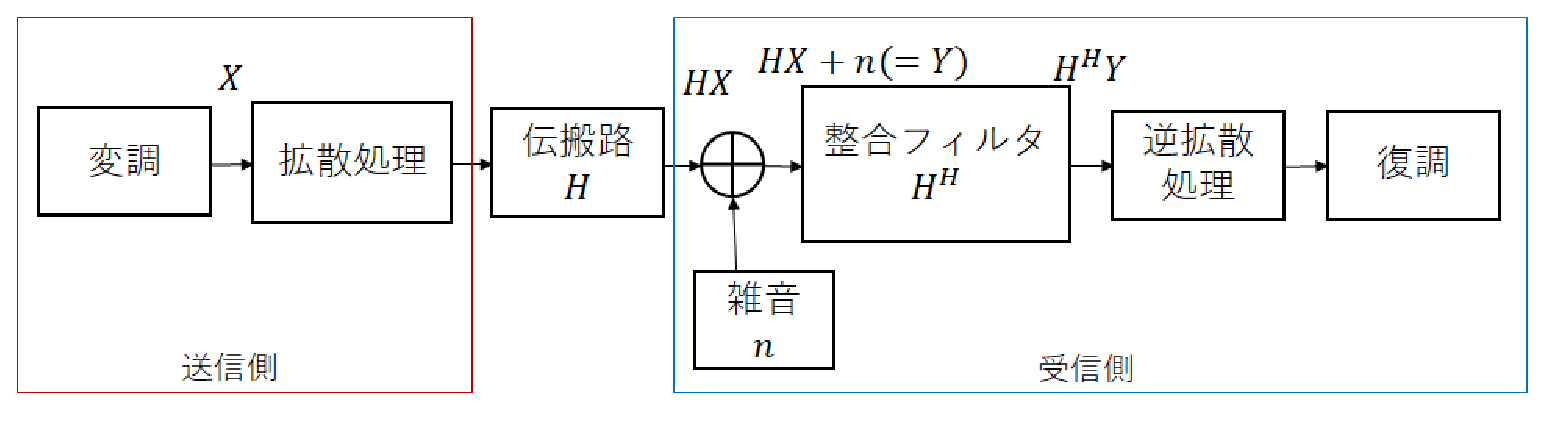
\includegraphics[width=\linewidth]{chapter2/figure/VC.eps}
    \caption{VC概略図}
    \label{figVC}
\end{figure}

\section{最適化問題の解法}
最適化問題は,与えられた制約条件の下で,目的関数と呼ばれる望ましさの尺度を表す関数が最小または最大となるような
決定変数の値を見つける,という数学モデルとして定式化できる. \cite{ibaragi}
最適化問題は,まず目的関数が線形関数か非線形関数かで大きく二つに分けることができる.そこからさらに,
制約条件の等号,不等号や決定変数が連続か非連続かによって細分化される.
一般に非線形関数の最適化の方が線形関数の最適化よりも困難とされる.

\subsection{KKT条件(Karush-Kuhn-Tucker condition)}
次のような不等式制約を持つ最適化問題を考える.

\begin{equation}
    \left\{
        \begin{array}{cc}
            目的関数:f(x) \to 最小 & \\
            制約条件:c_i(x) \leq 0 & (i=1,2,\ldots,m)
        \end{array}
    \right.
\end{equation}

ただし,変数$x$はn次元実ベクトルであり,目的関数$f:R^n \to R$および制約関数
$c_i:R^n \to R(i=1,\ldots,m)$はともに2回連続微分可能と仮定する.
まず,点$x$を(2.34)の実行可能解としたとき,$c_i(x)=0$が成り立つ制約条件を点$x$における有効制約
とよび,その集合を

\begin{equation}
    I(x) = {i| \quad c_i(x)=0 \hspace{10mm} (i=1,2,\ldots,m)} \nonumber
\end{equation}

で表す.さらに,有効制約の勾配ベクトル$\nabla c_i(x)(i \in I(x))$が1次独立であるような点$x$を
正則点という.

次の定理に示される条件は,非線形最適化問題の最適解を特徴づける重要な条件であり,KKT
(\emph{KKT: Karush Kuhn Tucker})条件と呼ばれる.\cite{ibaragi}

点$x^*$が(2.34)の局所的最適解かつ正則点ならば,

\begin{equation}
    \left\{
        \begin{array}{cccc}
            \nabla f(x^*)+\sum_{i=1}^m u_i^*\nabla c_i(x^*)=0 & & & \\
            c_i(x^*)\leq0, & u_i^*\geq0, & u_i^*c_i(x^*)=0 & (i=1,2,\ldots,m)
        \end{array}
    \right.
\end{equation}
を満たすベクトル$u^*=(u_1^*,u_2^*,\ldots,u_m^*)$が存在する.
ベクトル$u^*$をラグランジュ乗数と呼ぶ.

\subsection{ラグランジュの未定乗数法}
変数$\bm{x}$の関数$f(\bm{x})$の最大値,最小値は,等式制約$g(\bm{x})=0$が存在する場合,
ラグランジュ乗数$\lambda$を導入した

\begin{equation}
    F = f(\bm{x}) - \lambda g(\bm{x})
\end{equation}

を考え,これを$\bm{x}$で微分して$\bm{0}$と置く.

\begin{equation}
    \nabla_{\bm{x}}f - \lambda\nabla_{\bm{x}}g = \bm{0}
\end{equation}

これと等式制約$g(\bm{x})=0$を連立させて解けば,$\bm{x}$と$\lambda$を定めることができる.
この解法をラグランジュの未定乗数法と呼ぶ. \cite{kanatani}
ラグランジュの未定乗数法は線形最適化問題の解法として一般的である.
また,制約条件に不等式制約が存在する場合を考えるとき,ラグランジュの未定乗数法を
拡張した,2次計画法と呼ばれる解法が用いられる.
2次計画法を用いることでKKT条件の最適化問題を解くことができる.

\section{ディジタル変復調}
無線通信では,情報源のベースバンド信号(変調信号)を搬送波を用い,搬送波周波数帯の
信号に変換することが必要である.ベースバンド信号を伝送に適した形に変換することを変調と
呼び,逆の操作を復調と呼ぶ.これらの処理を合わせて変復調と呼び,その中でも情報源がディ
ジタルデータのものをディジタル変復調と呼ぶ\cite{takahata}.変調では,搬送波の振幅や周波数,位相な
どの性質を変化させることにより,信号を変換する.

\subsection{ディジタル変調}
\subsubsection{QPSK(Quadrature Phase Shift Keying)}
位相を用いて変調するものを位相偏移変調(PSK:Phase Shift Keying)と呼ぶ.
PSKでは,2進ディジタル信号を$n$ビットずつまとめ,これに対し$M=2^n$の位相を割り当てることで
搬送波に情報を持たせる.これを一般に$M$相PSKと呼び,
次の式で表される\cite{saitou}\cite{okumura}.
\begin{eqnarray}
\left\{
\begin{array}{ll}
\displaystyle s(t)=\mbox{Re}\left[Ae^{j(\omega_c t+\phi_m)}\right]&(-T/2 \leq t \leq T/2) \\[2mm]
\displaystyle \phi_m = \frac{2\pi}{M}(m-1) & (m=1,2, \cdots ,M)
\end{array}
\right.
\label{no2-6}
\end{eqnarray}
$M$相PSKの中でも$M$=4の場合を4位相偏移変調(QPSK:Quadrature Phase Shift Keying)と呼び,
$\phi_m=\pi/4,  3\pi/4,  5\pi/4,  7\pi/4$ が用いられる \cite{okumura}.
QPSK信号$S_{{\rm QPSK}}(t)$は,
\begin{eqnarray}
S_{{\rm QPSK}}(t)&=&\mbox{Re}\left[Ae^{j(\omega_c t +\phi_m)} \right] \nonumber \\
&=&\mbox{Re}\left[\left\{A\cos\phi_m+jA\sin\phi_m\right\}e^{j\omega_c t}\right] \nonumber \\[1mm]
&=&\mbox{Re}\left[\left\{Ad_1(t)+jAd_2(t) \right\}e^{j\omega_c t}\right] \nonumber \\[1mm]
&=&Ad_1(t)\cos\omega_ct-Ad_2(t)\sin\omega_ct
\label{eqqpsk}
\end{eqnarray}
と表される.ここで,
\begin{eqnarray}
\left\{
\begin{array}{ll}
\displaystyle \phi_m = \frac{2\pi}{4}(m-1)+\frac{\pi}{4} \hspace{2mm}(m=1,\cdots ,4) \\[2mm]
\displaystyle d_1 = \cos \phi_m \hspace{16mm}(=\pm1) \\[1mm]
\displaystyle d_2 = \sin \phi_m \hspace{16.5mm}(=\pm1)
\end{array}
\right.
\label{ff}
\end{eqnarray}
である.つまり,QPSKではこの4つの位相を2ビットの系列00,01,10,11に対応させて伝送する.
QPSK変調の信号点配置および,変調器の回路図を図\ref{fig:qpskIQ},図\ref{fig:qpskmod}に示す.
信号点配置はグレイコードが用いられ,隣接する信号点のハミング距離が1となるように設定されている.
%----------------------------画像をいれた----------------------------
\begin{figure}[t]
  \begin{center}
    \includegraphics[scale = 0.25]{./chapter2/figure/qpskiq.eps}
    \caption{QPSK変調の信号点配置の例}
    \label{fig:qpskIQ}
  \end{center}
\end{figure}
\begin{figure}[t]
  \begin{center}
    \includegraphics[scale = 0.25]{./chapter2/figure/qpskshift.eps}
    \caption{QPSK変調の回路図}
    \label{fig:qpskmod}
  \end{center}
\end{figure}

\subsection{同期検波}
変調された信号(被変調信号)から元の信号を得ることを復調という.復調方式として図 \ref{fig:qpskcoh} に示すような同期検波を考える.同期検波とは,変調側と同位相の搬送波を用い,受信信号との積をとることにより,元の変調信号を得る方法である\cite{takahata}.QPSK信号$S_{{\rm QPSK}}(t)$に$\cos\omega_c t$,$-\sin\omega_c t$をかけたものをそれぞれ$m_1(t), m_2(t)$とすると,
\begin{eqnarray}
m_1(t)&=&Ad_1(t)\cos^2\omega_ct+Ad_2(t)\sin\omega_ct\cos\omega_ct \nonumber \\
&=&\frac{1}{2}Ad_1(t)+\frac{1}{2}Ad_1(t)\cos2\omega_ct+\frac{1}{2}Ad_2(t)\sin2\omega_ct \\
m_2(t)&=&-Ad_1(t)\sin\omega_ct\cos\omega_ct+Ad_2(t)\sin^2\omega_ct \nonumber \\
&=&\frac{1}{2}Ad_2(t)-\frac{1}{2}Ad_2(t)\cos2\omega_ct-\frac{1}{2}Ad_1(t)\sin2\omega_ct
\end{eqnarray}
となる.ここで,$m_1(t)$,$m_2(t)$をローパスフィルタ(LPF:Low-Pass Filter)に通すことにより高周波成分を除いたものを$\hat{m}_1(t)$,$\hat{m}_2(t)$とすると,
\begin{eqnarray}
\hat{m}_1(t)&=&\frac{1}{2}Ad_1(t)\\
\hat{m}_2(t)&=&\frac{1}{2}Ad_2(t)
\end{eqnarray}
となる.$\hat{m}_1(t)$,$\hat{m}_2(t)$を並直列変換(parallel / serial conversion)することで,元の信号が復元される.
%------------------------------仮画像------------------------------
\begin{figure}[t]
  \begin{center}
    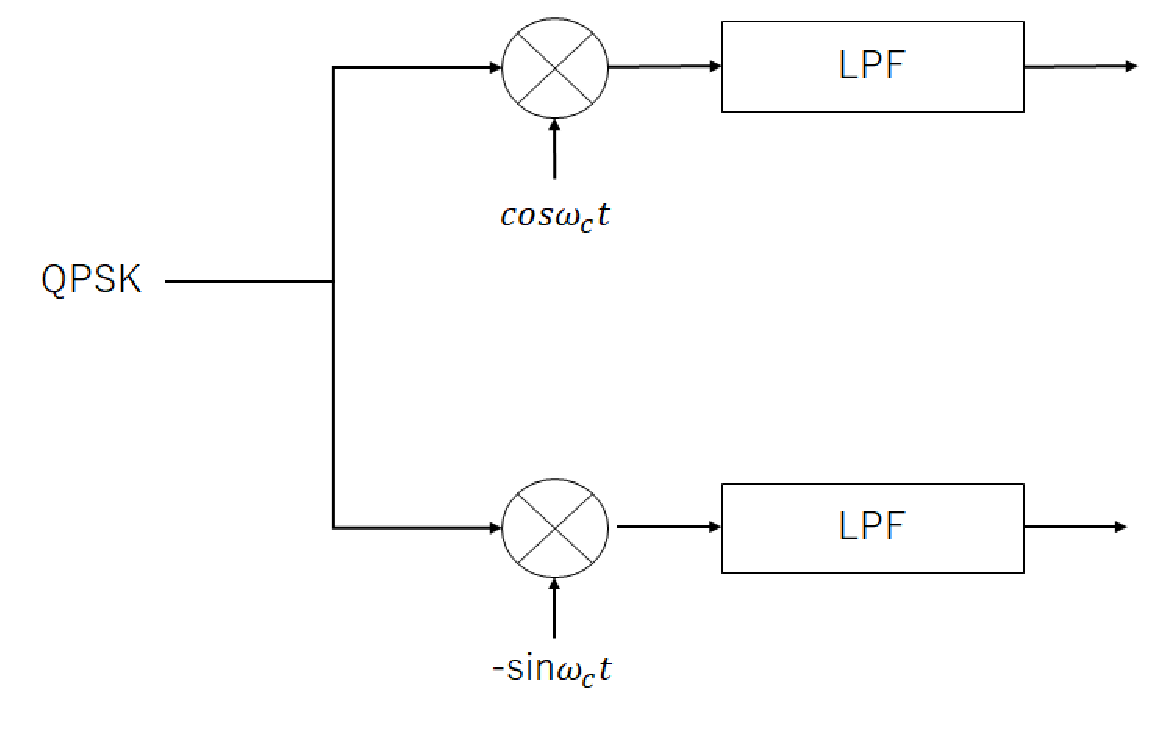
\includegraphics[scale = 0.25]{./chapter2/figure/douki.eps}
    \caption{QPSK変調の同期検波回路}
    \label{fig:qpskcoh}
  \end{center}
\end{figure}
%------------------------------------------------------------------

\subsection{信号の等価低域表現}
対象システムの特性をコンピュータシミュレーションのような離散時間処理によって評価する場合,サンプリング定理を満足するなるべく小さなサンプリング周波数を用い,演算量を削減することが望ましい.そこで本研究では,信号を複素ベースバンドで表現し,等価低域表現によるシミュレーションを行っている.

ここで,ベースバンド信号の帯域幅が$B[{\rm Hz}]$のQPSK変調信号を考える.搬送波の周波数が$f_c[{\rm Hz}]$である場合,信号の最高周波数が$f_c+B[{\rm Hz}]$となるため,標本化定理により,この信号は$2(f_c+B)[{\rm Hz}]$以上で標本化する必要がある.一方,式(\ref{eqqpsk})より,QPSK変調信号の複素数表現は,$\{Ad_1(t)+jAd_2(t)\}e^{j2\pi f_ct}$となる.複素数表現では,$f_c=0$として,複素ベースバンド信号で表すことができ,
\begin{eqnarray}
b(t)=Ad_1(t)+jAd_2(t)
\end{eqnarray}
となる.標本化定理から,$2B[{\rm Hz}]$以上でサンプリングすれば復調できるため,実信号表現の場合と比べてサンプリング周波数を低くすることができ,サンプル点数を減らすことができる.この表現方法を等価低域表現と呼ぶ\cite{takahata}.
%------------------------------------------------------------------------

\section{フェージング伝搬路の影響}
開空間を伝送媒体として用いる無線通信では,気象条件や地理的条件によってその伝搬路特性が変化する.
また,通信中に場所の移動が伴う場合は伝搬路特性の変動が更に厳しいものとなる.
この現象はフェージングと呼ばれ,送信信号に振幅変動や位相変動を発生させる.
その結果,受信信号の品質は顕著な影響を受ける \cite{saitou}.

\subsection{マルチパスフェージングの発生原理}
送信された電波は大気屈折率の変化や大地,山,建物,あるいは車等によって反射,回折,散乱する.
材質や入射角により,ある電波は大きな減衰を受け,ある電波はほとんど減衰せずに経路が変えられるなど
して,マルチパス伝搬路が形成される(図 \ref{fig:multipath}).

受信点では多数の波が干渉し,定在波が生じる.この中を移動すると到来する多数の波の干渉により
激しい振幅時間変動,位相時間変動が生じる.
この現象をフェージングと呼ぶ\cite{okumura}.
簡単な例として,複素搬送波$e^{j2\pi f_ct}$が伝送され,図 \ref{fig:coming_waves}のように,マルチパス伝搬路において複数の散乱波が受信される場合を考える.$n$番目のパスを通過した信号の振幅を$a_n(t)$,位相を$\theta_n(t)$とすれば,そのときの受信信号$r_n(t)$は,
\begin{eqnarray}
r_n(t)&=&{\rm Re}\left[a_n(t)e^{j2\pi f_c t+j\theta_n(t)}\right]\nonumber \\
&=&{\rm Re}\left[z_n(t)e^{j2\pi f_c t}\right]
\end{eqnarray}
となる.ここで$z_n(t)\equiv a_n(t)e^{j\theta_n(t)}$とし,$r_n(t)$の複素包絡線を表す.また,$a_n(t)$は複素包絡線$z_n(t)$の振幅変化,$\theta_n(t)$は複素包絡線$z_n(t)$の位相変化をそれぞれ表す.したがって,受信信号$r(t)$は,
\begin{eqnarray}
r(t)=\sum_{n=1}^{N}z_n(t)e^{j\pi f_ct}
\end{eqnarray}
となる.ここで,受信点や周囲の環境が静止している場合には,$a_n(t)$,$\theta_n(t)$はほとんど変化せず,準静的フェージングモデルを与える.一方,受信点が速度$v$で移動すると,到来角度$\phi_n$に応じて,$v\cos(\phi_n)/\lambda$のドップラー周波数変動を受け,動的フェージングモデルとなる.このとき,初期位相を$\varphi_n$とすると,$\theta_n(t)$は,
\begin{eqnarray}
\theta_n(t)=2\pi\frac{vt\cos\phi_n}{\lambda}+\varphi_n
\end{eqnarray}
となる.ここで,$v/\lambda=f_D$は最大ドップラー周波数といわれるものであり,物理的には移動局の進行方向($\phi_n=0$)からの到来波周波数が$f_D[{\rm Hz}]$だけ高くなるのに対して,後方($\phi_n=\pi$)からの到来波は$f_D[{\rm Hz}]$だけ低くなることを表す.
\begin{figure}[t]
  \begin{center}
    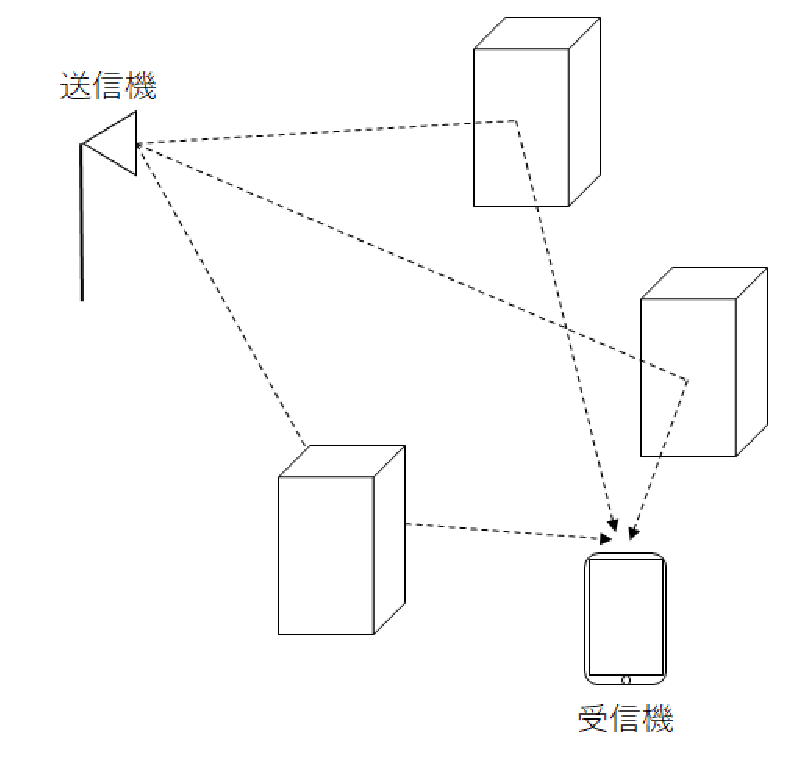
\includegraphics[scale = 0.25]{./chapter2/figure/multipaths.eps}
    \caption{マルチパス伝搬路モデル}
    \label{fig:multipath}
  \end{center}
\end{figure}

\begin{figure}[htbp]
	\begin{center}
		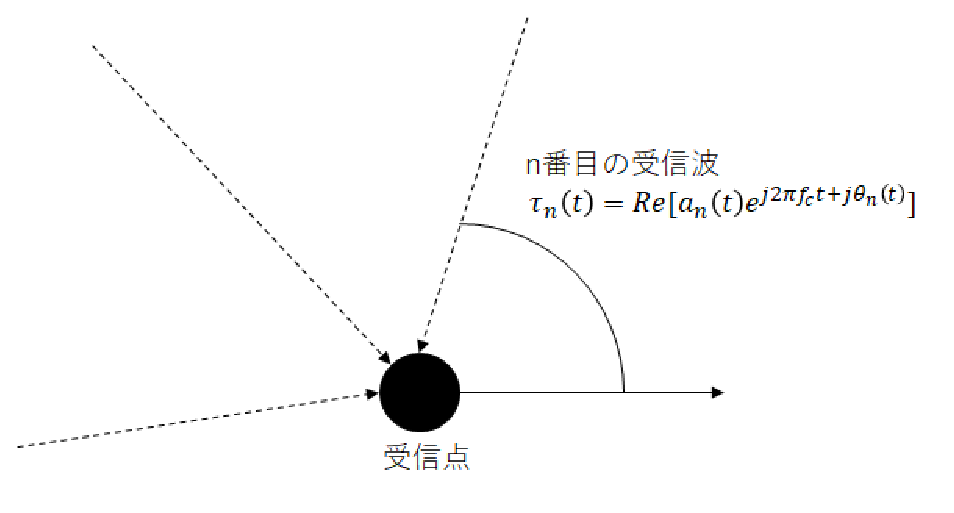
\includegraphics[scale=0.15]{./chapter2/figure/jushin.eps}
		\caption{マルチパス伝搬路の受信モデル}
		\label{fig:coming_waves}
	\end{center}
\end{figure}
%--------------------------------------------------------------------------------

\subsection{レイリーフェージング}
到来する素波数を$N$とする.このとき,受信信号$r(t)$の複素包絡線$z(t)$は,
\begin{eqnarray}
z(t)&=&\sum_{n=1}^{N}z_{n}(t) \nonumber \\
%&=&\sum_{n=1}^{N} a_{n}(t)e^{j\theta_{n}(t)} \nonumber \\
&=&\sum_{n=1}^{N}x_n(t)+j\sum_{n=1}^{N}y_n(t) \nonumber \\
&=& x(t)+j y(t)
\end{eqnarray}
となる.ここで,$x(t)$と$y(t)$はそれぞれ$z(t)$の同相成分,直交成分を表す.$x(t)$と$y(t)$は各波の強さが同程度である正弦波の和とすると,中心極限定理より$x(t)$,$y(t)$は平均値が0で等しい分散を持つ互いに独立な定常ガウス(Gauss)過程となる.$x=x(t)$,$y=y(t)$の結合確率密度関数$p(x,y)$は,
\begin{eqnarray}
p(x,y)=\frac{1}{2\pi \sigma^2}{\rm exp}\left(-\frac{x^2+y^2}{2\sigma^2}\right)
\end{eqnarray}
と表せる.ここで,$\sigma^2$は$r(t)$の平均受信電力である.包絡線振幅を$r$,位相を$\theta$とすると,
\begin{eqnarray}
\begin{cases}
r=\sqrt{x^2+y^2}& \\[4pt]
\theta=\tan^{-1}\left(\displaystyle \frac{y}{x}\right)&
\end{cases}
\end{eqnarray}
の関係がある.ここで,同相・直交成分の振幅が$(x, x+dx), (y, y+dy)$の領域に存在する確率は,デカルト座標から極座標に変換しても変わることはないため,次の式が成立する.
\begin{eqnarray}
\left\{
\begin{array}{ll}
p(x,y)dx\cdot dy & =p(r,\theta)dr\cdot d\theta  \\[12pt]
dx\cdot dy & =r\cdot dr\cdot d\theta
\end{array}
\right.
\end{eqnarray}
したがって,
\begin{eqnarray}
p(r,\theta)=\frac{r}{2\pi \sigma^2}{\rm exp}\left(-\frac{r^2}{2\sigma^2}\right)
\end{eqnarray}
となる.以上より,包絡線の確率密度関数$p(r)$と位相の確率密度関数$p(\theta)$は以下のように求められる.
\begin{eqnarray}
\left\{
\begin{array}{ll}
p(r)=\displaystyle \int_0^{2\pi}p(r,\theta)=\frac{r}{\sigma^2}{\rm exp}\left(-\frac{r^2}{2\sigma^2}\right)&(0\leq r \leq \infty)\\[12pt]
p(\theta)=\displaystyle \int_0^\infty p(r,\theta)dr=\frac{1}{2\pi} & (0\leq\theta\leq2\pi)
\end{array}
\right.
\end{eqnarray}
\begin{figure}[t]
	\begin{center}
		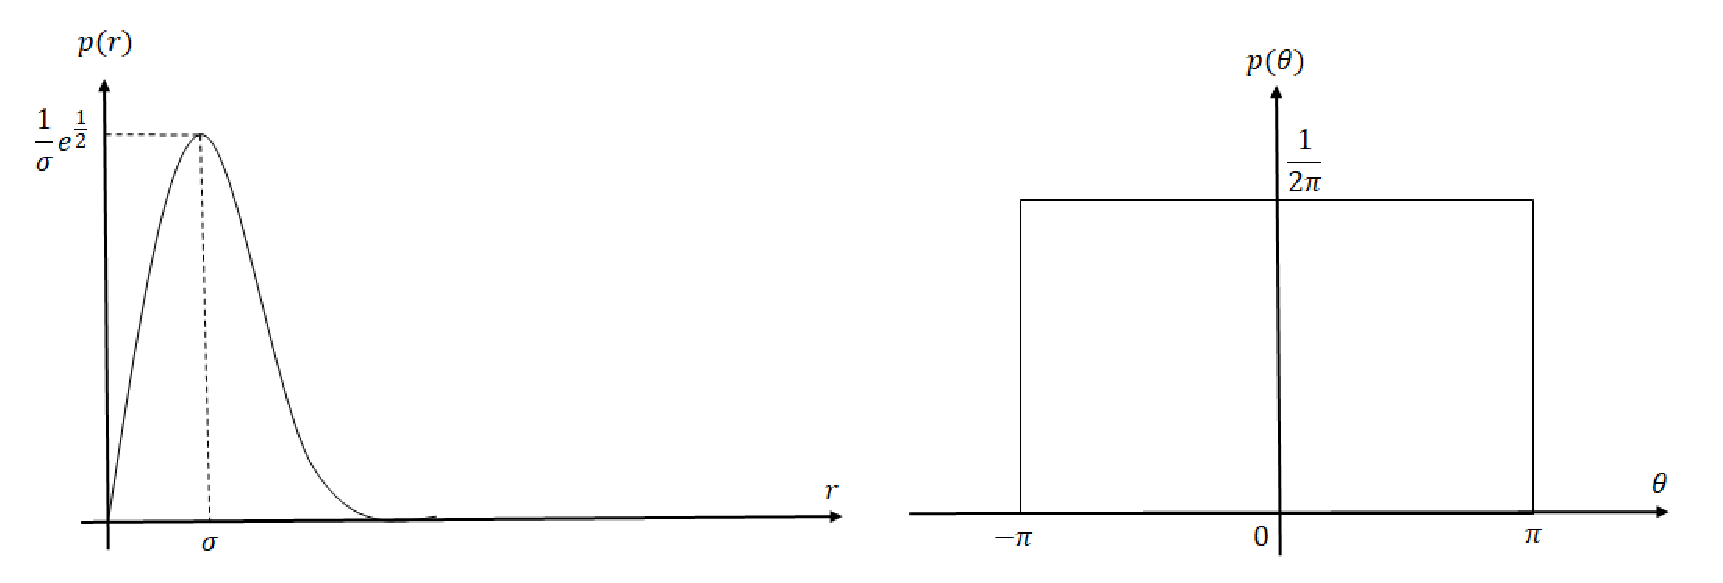
\includegraphics[scale=0.14]{./chapter2/figure/hourakusen.eps}
		\caption{包絡線と位相の確率密度関数}
		\label{figrayleigh}
	\end{center}
\end{figure}
$p(r)$,$p(\theta)$を図 \ref{figrayleigh}に示す.包絡線と位相の変動はそれぞれレイリー分布と一様分布に従うことがわかる.このようなフェージングをレイリーフェージングと呼ぶ\cite{saitou}\cite{okumura}.
%------------------------------------------------------------------------------ %基本的概念の解説
\chapter{Ping-Pong-Loopによる固有符号推定}

\section{ベクトル符号化}

\section{PPL(Ping-Pong-Loop)}

\section{復路のチャネルを$H^H$と見做すための非線形処理}

\section{合成チャネル行列の第1固有符号導出}

\section{合成チャネル行列の第2固有符号以降導出}
 %PPLアルゴリズム解説
\chapter{BER理論値を指標とする送信電力制御適用型使用チャネル足切りアルゴリズム
}
本章では,第3章で提案した既存のPPLアルゴリズムについて,研究背景,問題提起をしたのち,これに対する
改善案として3つの内容を検証する.1つ目に伝搬路のSN比が既知であるとしたときのBER理論値を基準とした
獲得固有ベクトル足切りアルゴリズム,2つ目に送信電力分配による理論BER最小化,そして3つ目に,
以上の2つの内容を同時適用した場合を検証する.

\section{研究背景}
第3章では,チャネル推定を行った後に合成チャネル行列を計算して固有値分解する
従来のVCに対して,べき乗法を基本原理とするPPLによる固有ベクトル獲得を提案した.
PPLの最大の特徴は,チャネル推定・合成チャネル行列計算・固有値分解の膨大な演算を,極めて簡単な
非線形処理と無線機間反復処理に置き換えることにある.つまり,伝搬路情報を経由せずに
直接的に固有値・固有ベクトルを求めることができる点に強みがある.
しかし,現在のPPLにおける固有値・固有ベクトルの獲得にかかる無線機間往復数では,実用には十分でないという
問題点がある.固有値問題の性質上,解法には反復解法を用いざるを得ない.PPLではべき乗法を
基本原理としているため,ある程度の反復回数の増加は避けられない.また,VCという方式自体としても
いくつかの課題を有している.その一つに,固有ベクトルに対応する固有値の大きさが,
そのままそのチャネルの利得になっているという特徴上,利得の小さい
チャネルを使用して伝送したデータが,他のチャネルを使用した場合と比較して誤りやすくなるという
問題がある.本章では,上記の二つの問題点に焦点を当て,3つの内容に分けて検証を行う.

\section{検討内容}
ここでは,全部で3つの内容について検討を行う.まず,1つ目としてPPLの課題である無線機間往復数に
対して,一定の通信品質を満たさないチャネルをBER理論値に基づいて足切りすることによる往復数削減
を検証する.2つ目に,VCの課題として挙げた低利得チャネルの誤り率増加減少に対して,送信電力制御
適用によるBER理論値最小化を行う.最後に,1つ目の足切りアルゴリズムに対して,送信電力制御を
組み込んだ場合について検証を行っていく.

\subsection{BER理論値を指標とする使用チャネル足切りアルゴリズム}
ここでは,BER理論値を指標とする使用チャネル足切りアルゴリズムについて解説を行う.
従来のPPLでは,反復処理を行う際,求めたい固有ベクトルの数をあらかじめ
決めたうえで,すべての固有ベクトルが収束するまで反復を行っている.しかし,これは反復回数の面
では無駄が多い.理由として主に以下の3つが挙げられる.1つ目に,べき乗法の特徴として,固有値を大きい順に並べた際に,隣の
固有値との比が大きいほど固有ベクトルの収束が速くなり,逆に小さいほど遅くなるという点が挙げられる.
つまり,求めたい固有ベクトルのうち小さい固有値に対応するものほど,必然的に前の固有値との
比が小さくなるため,獲得までに多くの反復回数を
要することになる.2つ目に,3.5節で説明したように,第2固有ベクトルの獲得では第1固有ベクトルを,
第3固有ベクトルの獲得では第1・第2固有ベクトルを必要とするように,
各固有ベクトルの獲得精度はそれ以前の固有ベクトルの獲得精度の影響を強く受ける.そのため,
後半になるにしたがって,固有ベクトルの獲得精度が低くなり,全体として見たとき拡散符号全体の
直交性が悪化してしまう.3つ目に,固有値が小さい,後半のベクトルほど誤り率が高くなるという
点が挙げられる.VCにおいて,固有値の大きさは各チャネルの利得に対応している.そのため,
固有値の小さいチャネルほど,受信される信号電力が低くなるので,SN比が低下し誤りやすくなるという
特徴がある.上記の理由から,小さい固有値に対応する後半の固有ベクトルを,適切に足切りする
ことができれば,実質的な通信品質を損なわずに不要な反復回数を削減できると考えられる.

図 \ref{figCutoff}に足切りアルゴリズムの概略図,図 \ref{figCutoffFlow}に足切りアルゴリズムのフローチャートを示す.
なお,図 \ref{figCutoff}の固有ベクトル導出に必要な処理は簡略版を示している.
\begin{figure}
    \centering
    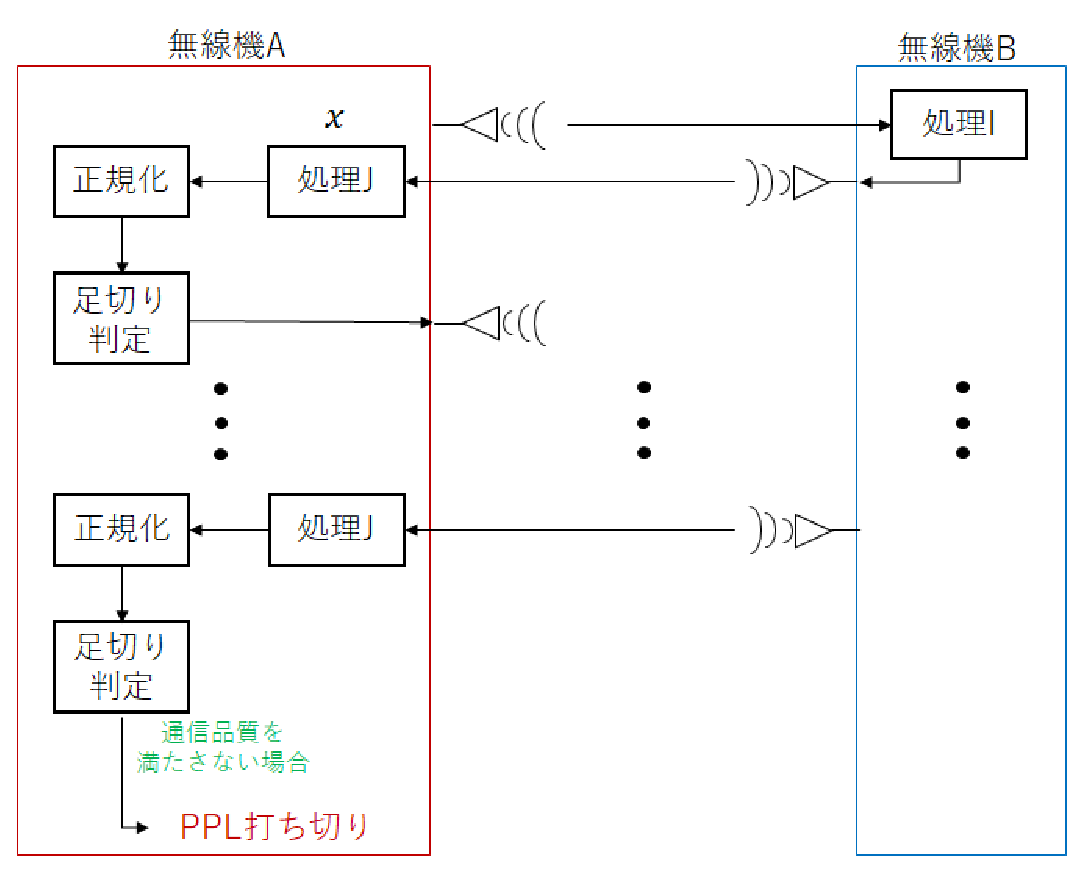
\includegraphics[width=\linewidth]{chapter4/figure/Cutoff.eps}
    \caption{足切りアルゴリズム概略図}
    \label{figCutoff}
\end{figure}
\begin{figure}
    \centering
    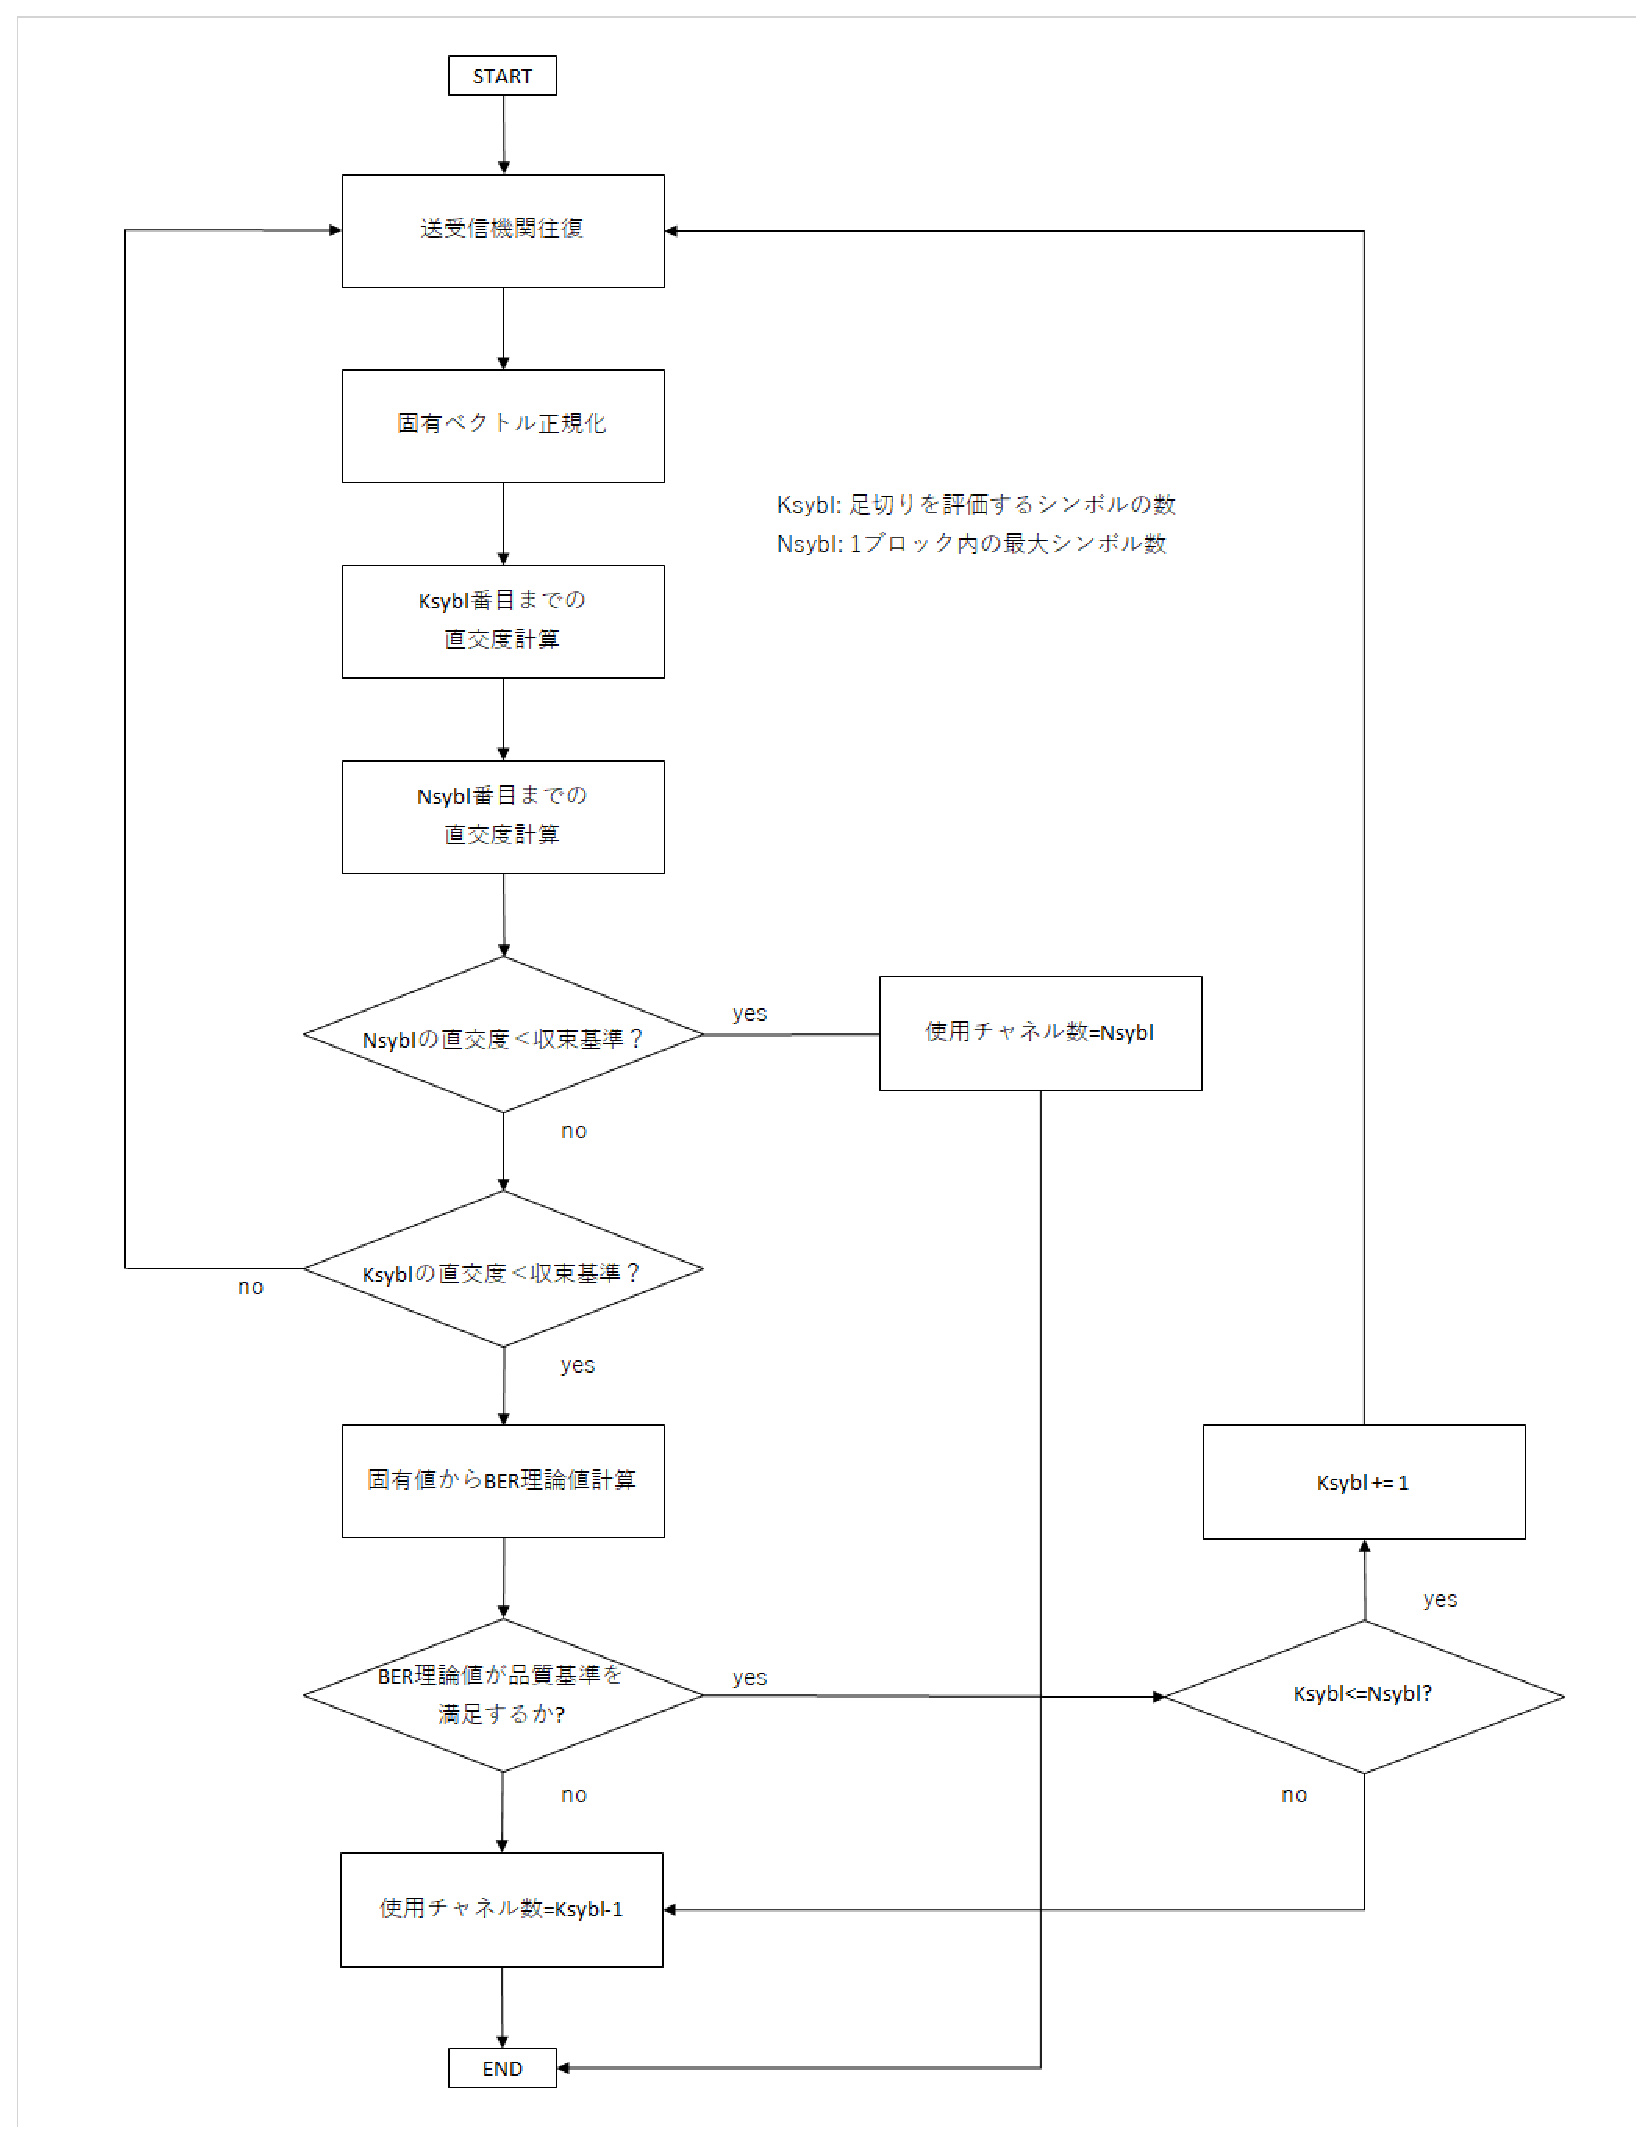
\includegraphics[width=0.95\linewidth]{chapter4/figure/CutoffFlow.eps}
    \caption{足切りアルゴリズムフローチャート}
    \label{figCutoffFlow}
\end{figure}
図 \ref{figCutoffFlow}のNsyblは最大獲得固有ベクトル数,Ksyblは足切り評価を行う固有ベクトル数に
なっている.また,固有ベクトルの収束判定基準に使用する直交度は以下のように定義するものとする.\\
\vspace{5mm}
(例) \quad 固有ベクトルが$\bm{u_1,u_2,u_3}$の3つの場合を考える.
\begin{equation}
    直交度 = \left|\bm{u_1^Hu_2}\right|+\left|\bm{u_1^Hu_3}\right|+\left|\bm{u_2^Hu_3}\right|
\end{equation}

具体的にどのように足切り判定が行われるか図 \ref{figCutoffFlow}をもとに説明する.
当該アルゴリズムは大きく分けて3つの段階に分かれている.
一つ目に無線機間往復,2つ目に獲得固有ベクトルの収束判定,そして3つ目に,収束した固有ベクトルを
用いた場合の通信品質がある基準を満たしているかのBER判定である.
まず,1つ目の無線機間往復について,これは第3章に説明したように非線形処理と正規化を伴う一連の
処理である.次に収束判定についてだが,これはKsybl番目までの固有ベクトルの直交度を求めて,
求めた値が事前に設定した収束基準を満たせば収束したとするものである.収束基準は実験的に求めた
値を使用する.
\begin{equation}
    Ksybl番目までの直交度 \leq 収束基準
\end{equation}
となれば,Ksybl番目までの固有ベクトルが求まったと判断する.
最後に,2つ目の収束判定を合格した固有ベクトルを使用した場合のBER理論値を計算し,
これがあらかじめ設定したBER基準を満たさなければ,Ksybl番目以降の固有ベクトルは獲得する必要がない
として無線機間往復を打ち切る.ここで,Ksybl番目までの固有ベクトルを使用する際の
BER理論値は以下の式,
\begin{equation}
    BER = \frac{1}{Ksybl}\sum_{i=1}^{Ksybl} \frac{1}{2}erfc\left( \sqrt{\lambda_i\frac{E_b}{N_0}} \right)
\end{equation}
で与えられる.上記のBER理論値はQPSKを変調方式として用いた場合のものである.
 \cite{akaiwa}なお,$erfc(x)$は相補誤差関数,$E_bN_0$は伝搬路の1ビット当たりの信号電力
対雑音電力比で,$E_bN_0$は既知とする.このBER理論値が,
\begin{equation}
    BER > BER基準
\end{equation}
を満たす場合,Ksybl番目を含めた通信品質が所望品質を満たさないとして,Ksybl-1番目までを
使用チャネルとしてPPLを打ち切る.ここで,BER基準は$10^{-2}$以下の誤り率であれば,
誤り訂正符号適用時に誤りを復元できるとして,$BER基準=10^{-2}$に設定する.
以上が当該アルゴリズムの解説になるが,1点補足として直交度の
計算部分にKsybl番目までとNsybl番目までの2通りの直交度を計算する部分がある.これは,
アルゴリズムの性質上Ksybl番目までの直交度よりNsybl番目までの直交度の方が早く収束する場合が
稀に存在するため,無線機間往復数が当該アルゴリズムを適用しない場合より増加しないようにするため
挿入している.

\subsection{送信電力制御を用いたBER理論値最小化}
ここでは,送信電力制御によるBER理論値最小化手法について解説を行う.
BER理論値の最小化は,各チャネルに割り当てられる送信電力を変数としたとき,目的関数である
BER理論値を最小とするような送信電力の組み合わせを見つける最適化問題を解くことで得られる.
以下で,式を用いて具体的に説明していく.

まず,変調方式にQPSKを使用する際のBER理論値は(4.3)式と同様に以下で表される.
\begin{equation}
    \frac{1}{N} \sum_{i=1}^N \frac{1}{2}erfc\left( \sqrt{\lambda_i\frac{E_b}{N_0}} \right)
\end{equation}
\begin{equation}
    \left[
        \begin{array}{l}
            N:1ブロック当たりのシンボル数 \\
            \lambda_i:i番目の固有ベクトルに対応する固有値 \\
            E_bN_0:平均E_bN_0
        \end{array}
    \right. \nonumber
\end{equation}
ここに,送信電力$p$を挿入することで,最小化する目的関数,
\begin{equation}
    f(p_1,p_2,\ldots,p_N) = \frac{1}{N} \sum_{i=1}^N \frac{1}{2}erfc\left( \sqrt{p_i\lambda_i\frac{E_b}{N_0}} \right)
\end{equation}
を得る.
また,送信電力$p_i$に関して,全送信電力の合計がNになるということと,各送信電力が非負であるので,
\begin{eqnarray}
    h(p_1,p_2,\ldots,p_N) = \sum_{i=1}^N p_i-N=0 \\
    p_i \geq 0 \hspace{10mm} (i=1,2,\ldots,N)
\end{eqnarray}
の2つの制約条件を考慮する必要がある.

\subsection{送信電力制御適用時の使用チャネル足切りアルゴリズム}

\section{検証}
\subsection{BER理論値を指標とする使用チャネル足切りアルゴリズム}
\subsubsection{シミュレーション諸元}
\subsubsection{シミュレーション結果}
\subsection{送信電力制御を用いたBER理論値最小化}
\subsubsection{シミュレーション諸元}
\subsubsection{シミュレーション結果}
\subsection{送信電力制御適用時の使用チャネル足切りアルゴリズム}
\subsubsection{シミュレーション諸元}
\subsubsection{シミュレーション結果}
 %提案手法解説・検証
\chapter{まとめ}
VCは,伝搬路と伝搬路の整合フィルタからなる合成チャネル行列の固有ベクトルを拡散符号と
するCDMである.
VCの拡散符号は,合成チャネル行列のエルミート性から互いに直交性を示す.すなわち,
送受信機において拡散・逆拡散処理を施すことによって,シンボル間干渉(ISI)を
生じさせることなく各変調信号を取り出すことが可能である.
また,受信機側に伝搬路に対する整合フィルタを置くことで,遅延派の取りこぼしのない
パスダイバーシチを実現することができる.この点において,遅延派の影響を削除する
OFDMと比較して優れた伝送特性を示すとされている.
固有ベクトルの獲得については,これまで伝搬路推定による方法が検討されて
きた.従来の方法では,まず伝搬路推定によって正確な伝搬路情報を獲得する必要が
あることと,伝搬路行列から合成チャネル行列の計算を行った後に固有値分解に
よって固有ベクトル必要があり,膨大な計算量が必要となる.そこで,本論文では
伝搬路推定や固有値分解の演算に代わって,ごく簡単な非線形処理と無線機間反復処理
によって逐次的に固有ベクトルを獲得するPPL(Ping-Pong-Loop)を提案している.
PPLは,演算能力の低い無線機でも簡単な無線機間反復処理によって固有ベクトルを
獲得することができる点をメリットとしているが,現状のアルゴリズムでは
多くの無線機間反復数を必要とするという課題があった.また,VC自体の課題として,
固有ベクトルに対応する固有値がチャネルの利得になることから,固有値が小さい
チャネルにおいて伝送する情報の誤り率が高くなってしまうという課題があった.
この2点の課題に焦点を当て,本論文ではこれらの問題の解決方法として3つの内容に対して
検討を行った.まず,1つ目として,無線機間反復数を削減する目的で,
獲得固有ベクトル足切りアルゴリズムを提案した.シミュレーションの結果から,
$E_bN_0$が小さい領域において,当該アルゴリズム適用した場合で無線機間反復数を
削減することができた.また,2つ目に,利得の小さいチャネルを救済するため,
BER理論値を目的関数,各チャネルに割り当てる送信電力を変数とする最適化問題を
解くことによってBER理論値を最小化できることを示した.
最後に3つ目として,足切りアルゴリズムに送信電力制御を適用することによって,
最低限必要なBER基準を満足するチャネル数を最大化しつつ,固有ベクトルの獲得に
必要な無線機間反復数を大きく削減できることを示した.将来的なPPLの展望としては,
現状では伝搬路の状態が頻繁に変化しない場合を想定しているが,
伝搬路の変化に合わせて既に獲得した拡散符号を追随して更新していく方式などに
検討の余地があると考える. %まとめ
\backmatter          %章番号をつけない          
\begin{thebibliography}{99}
    \bibitem{yamo} Y.Yamo, H.Suda, N.Umeda, and N.Nakajima,
    ``Radio Access Network Design Concept for the Fourth Generation Mobile
    Communication System,'' in Proc VTC'00-Spring, 2000,pp.2285-2289.

    \bibitem{pabst} R.Pabst et al, 
    “Relay based deployment concepts for wireless and mobile broadband radio,” IEEE
    Com.Mag, pp.80-89, Sep.2004

    \bibitem{kasturia} S.Kasturia, J.T.Aslanis, and J.M.Cioffi, ``Vector coding for partial
    response channels'', IEEE Trans. On Information Theory, Vol36, No.4, July 1990.

    \bibitem{furukawa} 古川, ``符号の直交分離とパスダイバーシチを同時に表現する符号分割多重伝送'',
    信学技法, RCS2006-52, 2006年8月

    \bibitem{li} Z.Li and H.Furukawa, ``An enhanced vector coding and its application to delay
    spread MIMO channels'', Proc. IEEE APWCS2007, Aug, 2007.

    \bibitem{takeda} 竹田, 中川, ``Vector CodingとOFDMの性能比較に関する検討'', 信学技法,
    RCS2007-215, March 2008.

    \bibitem{takanashi} 高梨, 竹田, 安達, 中川, ``Vector Coding における送信ダイバーシチの適用効果に
    関する一検討'', 信学技法, RCS2008-49, 2008年7月.

    \bibitem{takano} 高野 , 安達 , 大槻 , 中川, ``チャネル推定誤差及びフィードバック遅延を考慮したVC伝送
    系における送受信重み選択に関する理論検討'', 信学技法, RCS2010-13, 2010年4月.

    \bibitem{takeda2} D.Takeda, Member and M.Nakagawa, ``Adaptive Modulation and Code channel
    Elimination for Vector Coding System'', IEICE Trans Commun. Vol.E92-B, No.5, May.2009.

    \bibitem{nagate} 長手厚史, 舛井淳祥, 藤井輝也, ``OFDM方式におけるチャネル推定方に関する一検討''
    , 信学技法, RCS2001-195, pp.85-91, January 2002.

    \bibitem{imamura} 今村大地, 原晋介, 森永規彦, ``パイロット信号を用いたOFDMにおける副搬送波再生法'',
     電子情報通信学会論文誌 B , Vlo.J82-B, No.3, pp.393-401, 1999年3月.

    \bibitem{strang} G.ストラング, ``線形代数とその応用'', 産業図書株式会社, 2009.

    \bibitem{ibaragi} 茨木俊秀, 福島雅夫, ``最適化の手法'', 共立出版株式会社, 1993.

    \bibitem{kanatani} 金谷健一, ``線形代数セミナー 射影, 特異値分解, 一般逆行列'', 共立出版株式会社, 2018.

    \bibitem{takahata} 高畑文雄, ``ディジタル無線通信入門'', 培風館, 2002.

    \bibitem{saitou} 斉藤洋一, ``ディジタル無線通信の変復調'', 電子情報通信学会, 1996.

    \bibitem{okumura} 奥村喜久, 進士昌明, ``移動通信の基礎'', 電子情報通信学会, コロナ社, 1996.

    \bibitem{akaiwa} 赤岩芳彦, ``ディジタル移動通信技術のすべて'', コロナ社, 2013.
\end{thebibliography}
 %参考文献
\chapter{謝辞}
 %謝辞
%\include{付録}
\end{document}